

\section{Method}

TODO


% TODO:  replace the following rows
%\toprule
%OpenML ID &                Name &  \# Instances &  \# Num. Features &  \# Cat. Features \\
%\midrule

%TODO with this and move the caption to the bottom
%\toprule
%\multirow{2}{*}{OpenML ID} & \multirow{2}{*}{Name} & \multirow{2}{*}{Instances} & \multicolumn{2}{c}{Features} \\ \cline{4-5}
%\\[-0.75em]
%&                       &                            & Numerical    & Categorical   \\
%\midrule

\begin{table}[h!]
\centering
\begin{tabular}{rllrrr}
\toprule
\multirow{2}{*}{OpenML ID} & \multirow{2}{*}{Name} &\multirow{2}{*}{To-be-imputed Column} & \multirow{2}{*}{Obs.} & \multicolumn{2}{c}{Features} \\ \cline{5-6}
\\[-0.75em]
&                     &  &                            & Num.    & Cat.   \\
\midrule
     42545 &  stock\_fardamento02 &  Material &        6277 &                6 &                1 \\
     42675 &        auml\_eml\_1\_d &   F4\_plsa\_topic\_10 &      4585 &               11 &                0 \\
       198 &     delta\_elevators &   curRoll &      9517 &                7 &                0 \\
     23515 &              sulfur &     a3 &   10081 &                7 &                0 \\
       189 &              kin8nm &     theta8 &    8192 &                9 &                0 \\
       287 &        wine\_quality &    sulphates &     6497 &               12 &                0 \\
     42636 &                Long &     x18 &    4477 &               20 &                0 \\
     42688 &    Brazilian\_houses &   area &     10692 &                9 &                4 \\
     42183 &       dataset\_sales &   day &     10738 &               15 &                0 \\
      1199 &     BNG(echoMonths) &   wall\_index &     17496 &                7 &                3 \\
       197 &             cpu\_act &    pgin &     8192 &               22 &                0 \\
       218 &            house\_8L &    P3 &    22784 &                9 &                0 \\
     42712 & Bike\_Sharing\_Demand &   humidity &     17379 &                9 &                4 \\
      1193 &         BNG(lowbwt) &    UI &    31104 &                3 &                7 \\
       216 &           elevators &    climbRate &    16599 &               19 &                0 \\
       215 &            2dplanes &    x6 &    40768 &               11 &                0 \\
     23395 &     COMET\_MC\_SAMPLE &   wire\_id &     89640 &                6 &                0 \\
     42225 &            diamonds &    carat &    53940 &                7 &                3 \\
      1200 &          BNG(stock) &  company1 &      59049 &               10 &                0 \\
      1213 &             BNG(mv) &    x5 &    78732 &                8 &                3 \\
     42669 &          auml\_url\_2 &   mld.ps\_res &     95911 &               13 &                0 \\
\bottomrule
\end{tabular}
\caption{Overview of all data sets we use associated with a regression downstream task. \emph{To-be-imputed Column} presents the data set's column we used to evaluate the imputation methods, \emph{Obs.} the number of observations, \emph{Num.} the number numerical columns, and \emph{Cat.} the number of categorical columns.}
\label{tab:regression_data}
\end{table}

\begin{table}[h!]
\centering
\begin{tabular}{rllrrr}
\toprule
\multirow{2}{*}{OpenML ID} & \multirow{2}{*}{Name} & \multirow{2}{*}{To-be-imputed Column} & \multirow{2}{*}{Obs.} & \multicolumn{2}{c}{Features} \\ \cline{5-6}
\\[-0.75em]
&                       &                    &        & Num.    & Cat.   \\
\midrule
       737 &                       space\_ga & INCOME &         3107 &                6 &                1 \\
       871 &                         pollen &     RIDGE &    3848 &                5 &                1 \\
     40983 &                           wilt &    Mean\_G &     4839 &                5 &                1 \\
       728 &            analcatdata\_supreme &    Lower\_court\_disagreement &     4052 &                7 &                1 \\
      1489 &                        phoneme &     V1 &    5404 &                5 &                1 \\
       803 &                 delta\_ailerons &   RollRate &      7129 &                5 &                1 \\
       923 &               visualizing\_soil &     isns &    8641 &                3 &                2 \\
       725 &                        bank8FM &     a2pop &    8192 &                8 &                1 \\
     42192 &               compas-two-years &   age &      5278 &                7 &                7 \\
      1558 &                 bank-marketing &    V7 &     4521 &                7 &               10 \\
       310 &                    mammography &   attr2 &     11183 &                6 &                1 \\
      1046 &                       mozilla4 &    end &    15545 &                5 &                1 \\
       847 &                           wind &      year &   6574 &               14 &                1 \\
     40701 &                          churn &    total\_day\_minutes &     5000 &               16 &                5 \\
     41146 &                        sylvine &     V4 &    5124 &               20 &                1 \\
      1496 &                       ringnorm &     V4 &    7400 &               20 &                1 \\
      1507 &                        twonorm &     V5 &    7400 &               20 &                1 \\
       823 &                         houses &     total\_rooms &   20640 &                8 &                1 \\
     42493 &                       airlines &     Length &   26969 &                2 &                6 \\
      1471 &                  eeg-eye-state &    V9 &    14980 &               14 &                1 \\
      1120 &                 MagicTelescope &    fAlpha: &    19020 &               11 &                1 \\
      4135 &         Amazon\_employee\_access &    MGR\_ID &    32769 &                0 &               10 \\
       137 &               BNG(tic-tac-toe) &    top-middle-square &    39366 &                0 &               10 \\
       251 &                  BNG(breast-w) &   Cell\_Shape\_Uniformity &     39366 &                9 &                1 \\
      1220 &         Click\_prediction\_small &    keyword\_id &    39948 &                9 &                1 \\
       151 &                    electricity &   nswprice &     45312 &                7 &                2 \\
       901 &                          fried &    X2 &    40768 &               10 &                1 \\
       881 &                             mv &   x3 &     40768 &                7 &                4 \\
     40922 &        Run\_or\_walk\_information &   gyro\_y &     88588 &                6 &                1 \\
     42477 & default-of-credit-card-clients &   x1 &     30000 &               23 &                1 \\
     23517 &                    numerai28.6 &     attribute\_10 &   96320 &               21 &                1 \\
\bottomrule
\end{tabular}
\caption{Overview of all data sets we use associated with a binary classification downstream task. \emph{To-be-imputed Column} presents the data set's column we used to evaluate the imputation methods, \emph{Obs.} the number of observations, \emph{Num.} the number numerical columns, and \emph{Cat.} the number of categorical columns.}
\label{tab:binary_data}
\end{table}

\begin{table}[h!]
\centering
\begin{tabular}{rlrrr}
\toprule
\multirow{2}{*}{OpenML ID} & \multirow{2}{*}{Name} & \multirow{2}{*}{Observations} & \multicolumn{2}{c}{Features} \\ \cline{4-5}
\\[-0.75em]
&                       &                            & Numerical    & Categorical   \\
\midrule
      1526 &                  wall-robot-navigation &         5456 &                4 &                1 \\
       183 &                                abalone &         4177 &                7 &                2 \\
     40498 &                     wine-quality-white &         4898 &               11 &                1 \\
        30 &                            page-blocks &         5473 &               10 &                1 \\
     40677 &                                  led24 &         3200 &                0 &               25 \\
      1459 &                  artificial-characters &        10218 &                7 &                1 \\
     40497 &                            thyroid-ann &         3772 &               21 &                1 \\
      4552 &                      BachChoralHarmony &         5665 &                2 &               15 \\
        26 &                                nursery &        12960 &                0 &                9 \\
       375 &                         JapaneseVowels &         9961 &               14 &                1 \\
        32 &                              pendigits &        10992 &               16 &                1 \\
      1481 &                                kr-vs-k &        28056 &                3 &                4 \\
       184 &                                  kropt &        28056 &                0 &                7 \\
     41027 & jungle\_chess\_2pcs\_raw\_endgame\_complete &        44819 &                6 &                1 \\
         6 &                                 letter &        20000 &               16 &                1 \\
     41671 &                      microaggregation2 &        20000 &               20 &                1 \\
     40685 &                                shuttle &        58000 &                9 &                1 \\
\bottomrule
\end{tabular}
\caption{Multiclass classification datasets.}
\label{tab:multiclass_data}
\end{table}




Datasets from OpenML:
Using \code{openml} python library to retrieve all available datasets. Filter for the following properties:
\begin{itemize}
	\item 3k to 100k observations
	\item 5 to 25 features
	\item no missing values (necessary to get ground truth)
\end{itemize}

We than removed some obvious duplicated and corrupted datasets by hand and omit datasets of the Sparse ARFF format. This leads to 70 datasets, 22 regression tasks, 31 binary classification, and 17 multi-class classification tasks.

Here or in supplemental material: Table with all dataset IDs and basic statistics (number of rows, number of categorical columns, number of numerical columns, TODO?)


\subsection{Imputation Methods}
%
Implement uniform interface inspired by \emph{scikit-learn}\footnote{TODO Link}: fit and transform. Where fit trains the imputer on the given \code{DataFrame} to impute the given \code{target columns}  and optimizes hyperparameters on at least 3 folds. On the other hand, \code{transform} fills the missing values in the trained \code{target columns} in the given \code{DataFrame}. Figure \label{imputer_process} this.
%
\begin{figure}[h!]
	\centering
	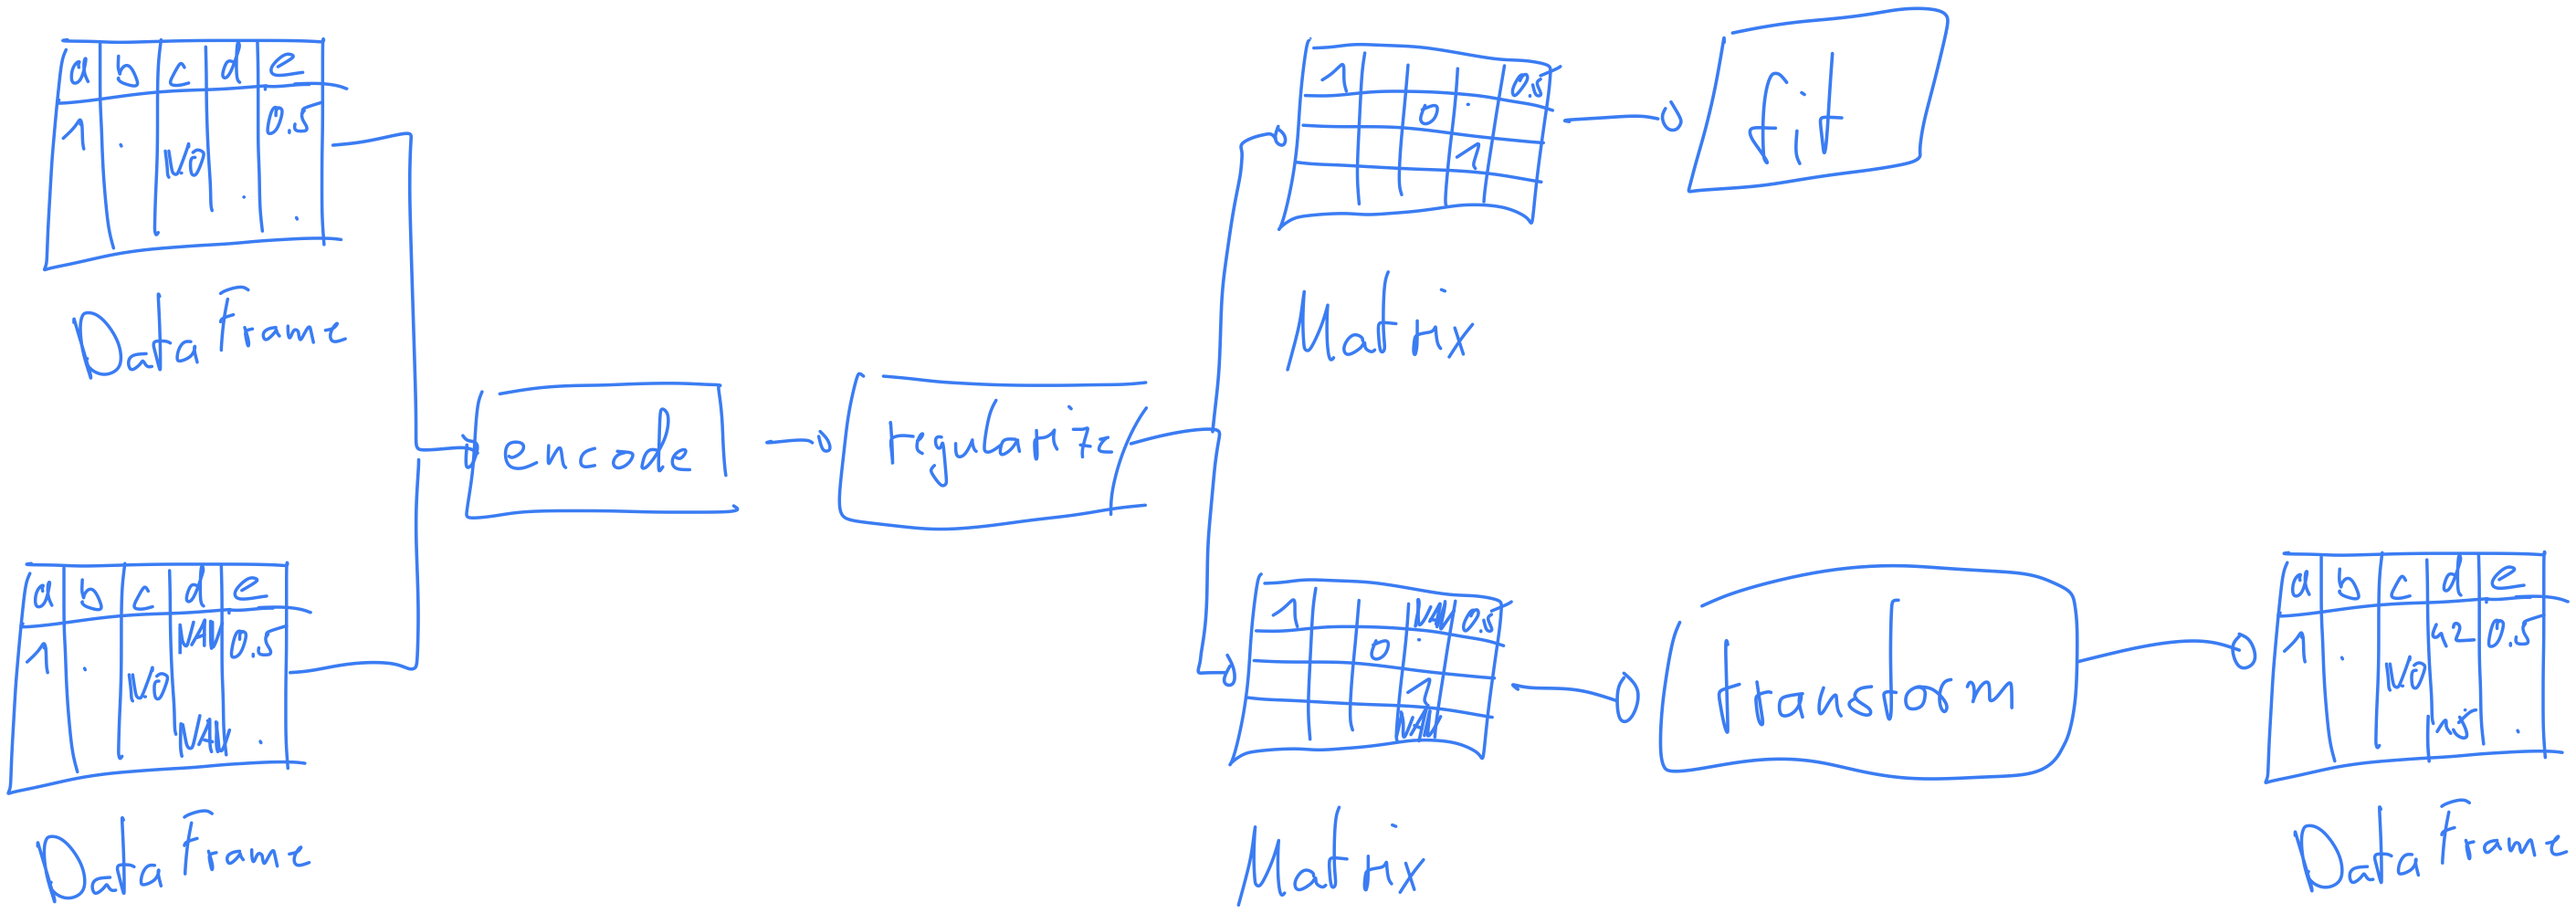
\includegraphics[width=10cm]{figures/fit_process}
	\caption{TODO}
	\label{fig:imputer_process}
\end{figure}

TODO: Irgendwo, muss hin, dass wir GridSerach nutzen für HPO..

\subsubsection{Simple Imputer}
%
Uses the column-wise \code{mean} for numerical or \code{mode}, i.e., the most frequent value,  for categorical columns to fill missing values.


\subsubsection{Machine Learning-based Imputer}
%
Two representatives here: \emph{K-NN Imputer} and \emph{Random Forest Imputer}. We build \code{scikit-learn}\footnote{TODO version} pipeline that models the \code{target columns} over all other available columns. The encoding step (see figure \ref{imputer_process}) first mark all missing values with the column's mean for numerical columns and the most frequent value for categorical ones. Second, it encodes the categorical columns as one-hot, and third, standardize  the matrix (rescale to zero mean and unit variance).

Depending on the \code{target column}'s datatype (categorical or numerical), we use \code{scikit-learn}'s \code{KNeighborsClassifier} and \code{KNeighborsRegressor} for K-NN Imputer, or \code{RandomForestClassifier} and \code{RandomForestRegressor} for Random Forest Imputer.


\subsubsection{Deep Learning-based Imputer}
%
For deep learning models, we need to consider the number of layers and neurons per layer as hyperparameters to properly optimize the model. This is why we use \code{autokeras}\cite{AutoKeras} to build our \code{Deep Learning Imputer}. AutoKeras is an AutoML framework that tries automatically different model architectures.

Similar to our ML-based imputer, we use \code{autokeras}' \code{StructuredDataClassifier} for categorical target columns or \code{StructuredDataRegressor} for numerical columns. However, we do not need to take care of encode the data since \code{autokeras} automatically handle this.


\subsubsection{Generative Imputer}
%
Since generative models estimate the data distribution and can generate similar distributions\cite{Generativ_survey}, it stands to reason that they are used to impute missing values. Common approaches are variational auto encoders (VAE) (TODO: cites) and generative adversarial networks (TODO: cites), which is why we used for both one representative method.

\paragraph{Generative Adversarial Imputation Nets (GAIN)}
%



\paragraph{Variational Auto Encoder (VAE)}
%
